\textcolor{red}{[additional motivation for coala memory virtualization] we should emphasize that Coala programming model removes the burden of identifying the write-after-read dependencies from the programmer  as compared to Chain. And it does not require a specific compiler that cannot consider a runtime dependent behavior like Interrupts service handling to guarantee memory protection, as in Alpaca.}

\sys's {\em virtual memory manager} exposes non-volatile memory for
\emph{protected} variables to the application as a virtual address space
partitioned into pages.  
%
A program's tasks read and write these protected variables, using them like any
other data in the program. 
%
The virtual memory manager automatically finds a variable in its page and  
allows a task to directly manipulate its value.
%
When a task completes, the virtual memory manager ensures that updated pages 
are committed to main memory and visible to subesequently executed tasks.
%
If a power failure interrupts a task, the virtual memory manager ensures that
the task sees consistent memory state when it restarts its execution. 
%
The virtual memory manager ensures consistency even if a task or a sequence of tasks include WAR dependences that could compromise consistency~\cite{ratchet,dino}.
%
%
%
%,. Virtualization simplifies
%coalescing, because the system gets the freedom to move application's data
%between volatile and non-volatile memory transparently.
%

\sys's virtual memory manager \sys abstracts non-volatile storage (e.g.,
variables in FRAM) from tasks, which simply manipulate protected variables.
%
Protected variables remain consistent and are durable across power failures.
%
While ensuring variables remain durable, \sys avoids accessing non-volatile
memory when possible, by copying pages of data into a {\em working memory} in the device's SRAM, which
has a lower latency and energy cost to access than the device's FRAM (as we
showed in Section~\ref{sec:background}).
%
%
On a commit, \sys atomically copies all updated (i.e., ``dirty'') pages from their
space in the working memory back into their location in the non-volatile
memory.
%
SRAM has a limited size and there is an extended working memory containing {\em
shadow pages} in the larger FRAM.  A shadow page stores the data from an
updated pages that need to be committed back to non-volatile memory, but that
exceeded the size of the volatile working memory. 
%
%manages memory such that application tasks operate primarily from
%efficient volatile SRAM rather than non-volatile FRAM, which is more costly to access than SRAM,
%as we showed in Figure~\ref{fig:framEnergy}. 
\sys moves pages of data efficiently using hardware accelerated Direct Memory
Access (DMA) support, which copies a block of memory from one place to another
as a single operation. 


\begin{figure}
	\centering
	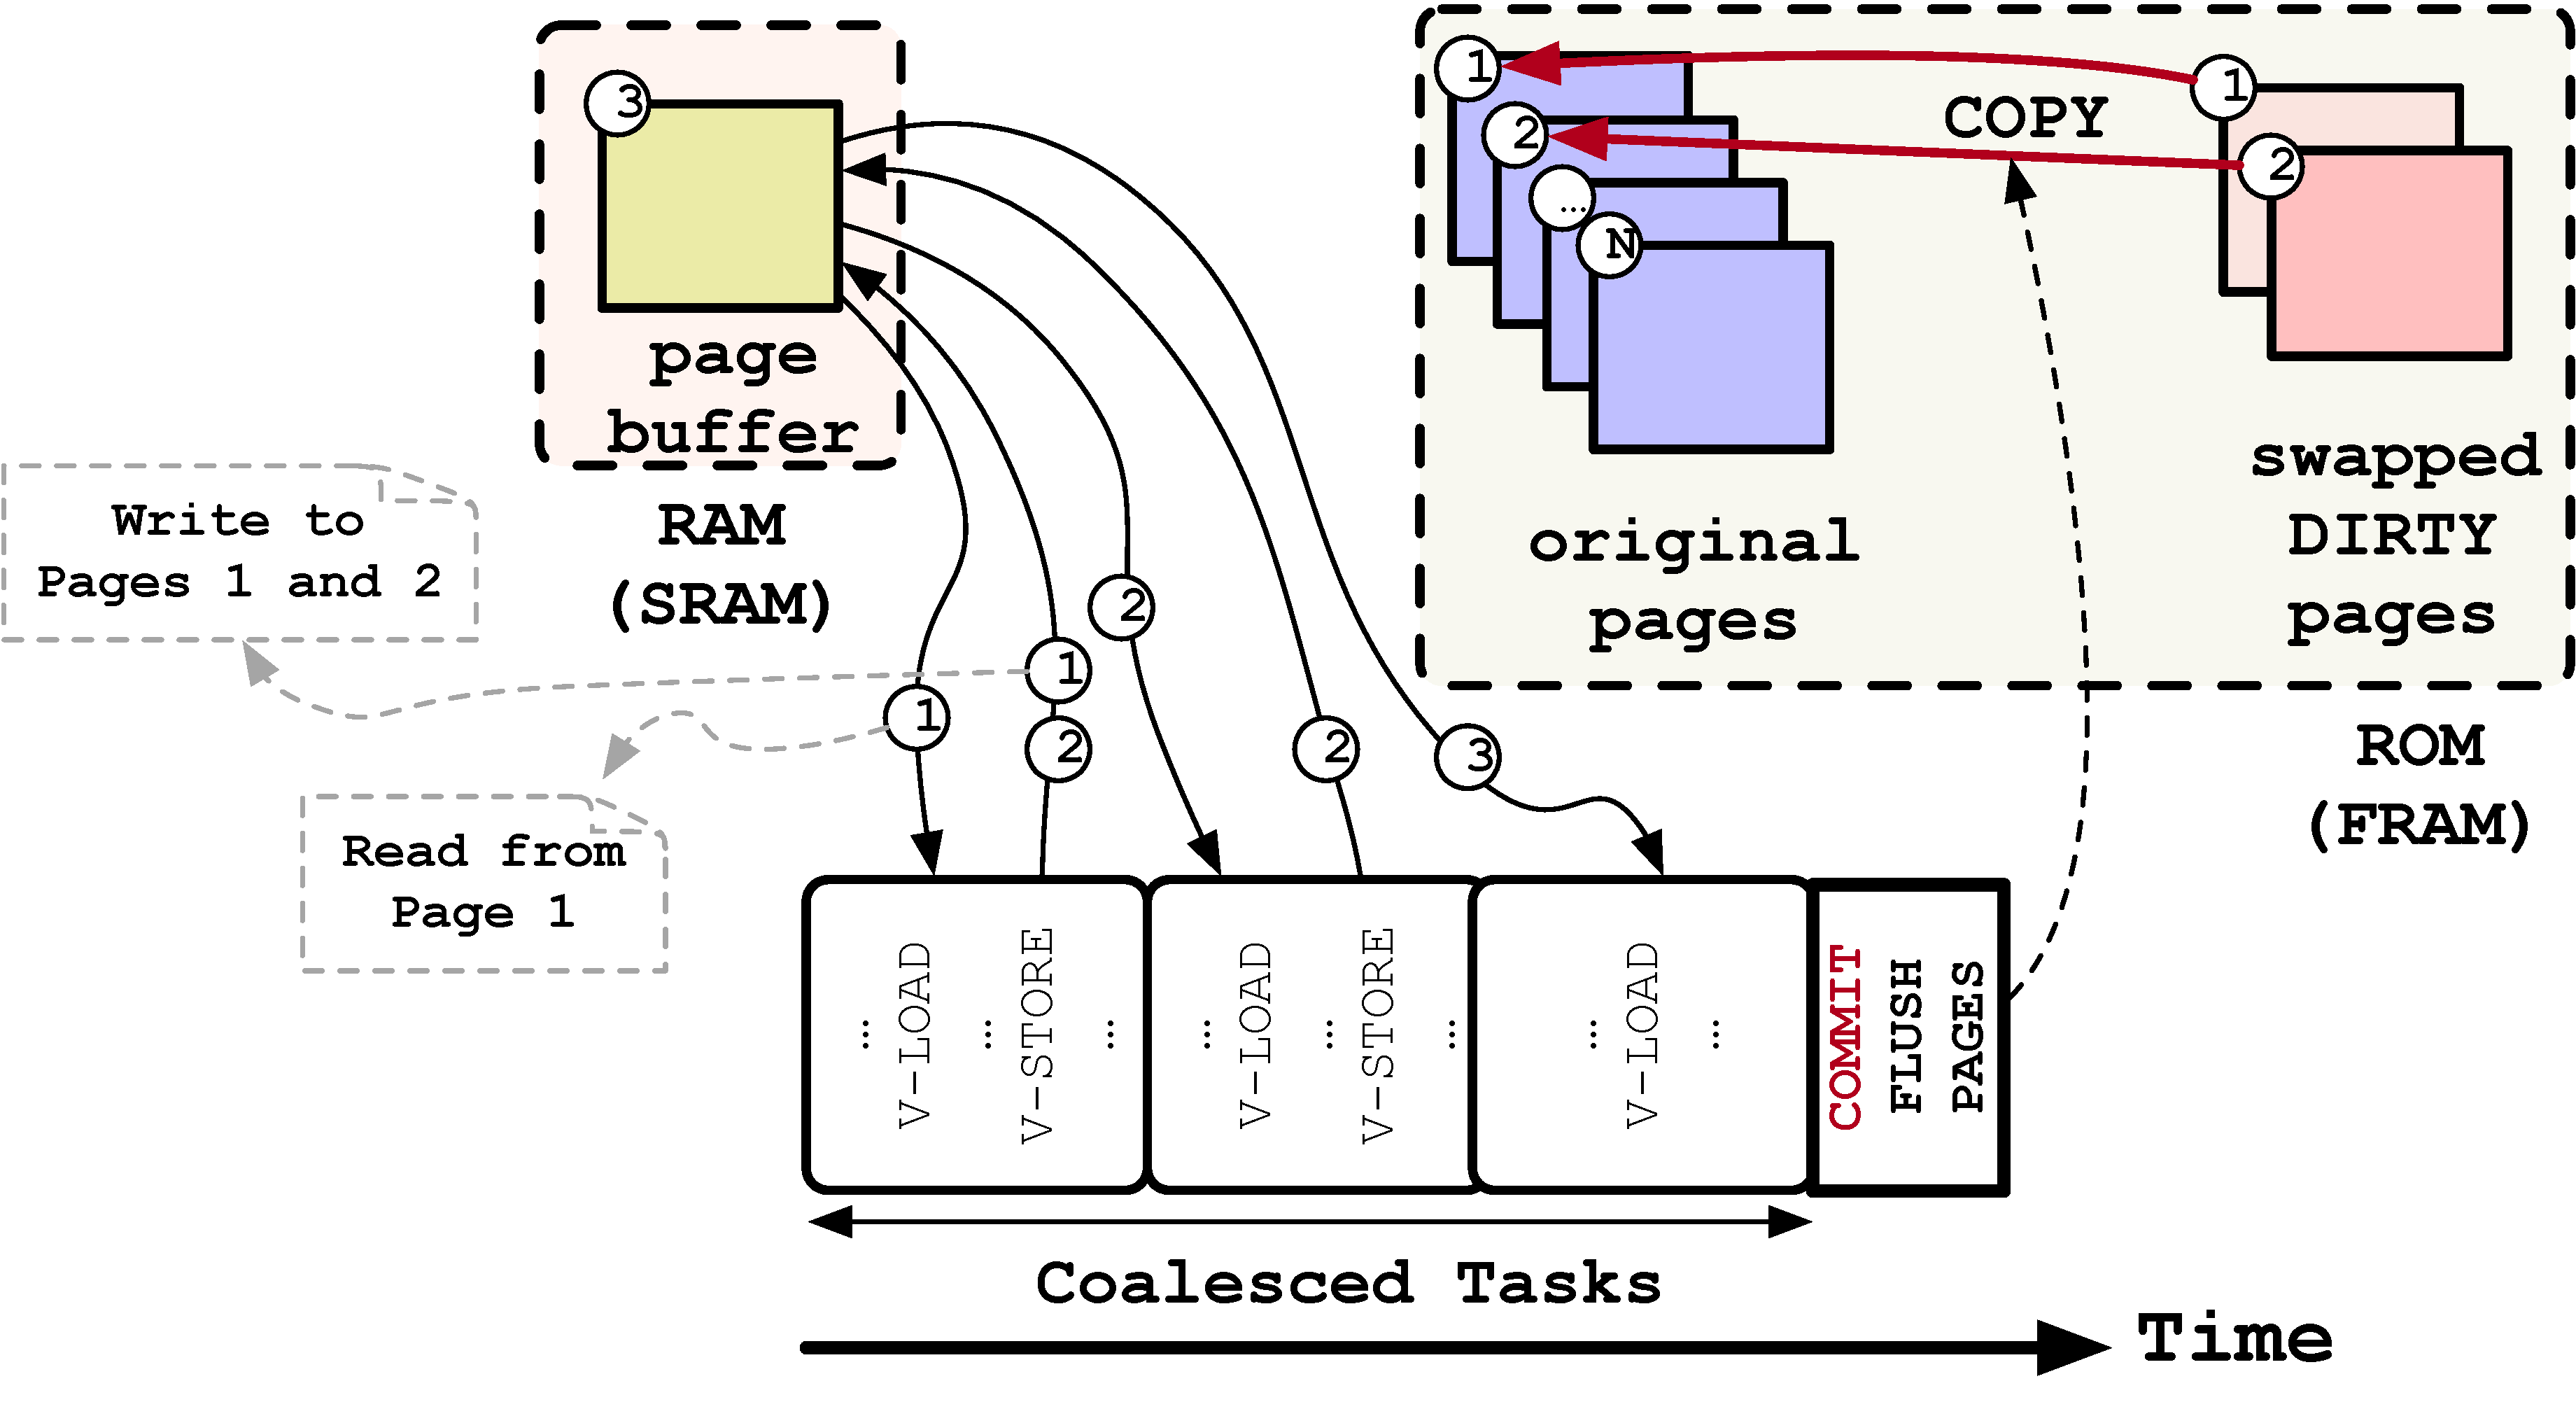
\includegraphics[width=\textwidth]{figures/graffle/paging.pdf}
	\caption{Illustration of task-virtual memory interaction in \sys. Tasks only interact with the working buffer in SRAM (indicated as page buffer). The shadow buffer is used to hold the dirty bages. The indirection table is used to speed-up two-phase commit operation: it eliminates the copy operation in the second phase.}
	\label{figure:coala_page_tags}
\end{figure}

\textbf{System Overview.} Figure~\ref{figure:coala_page_tags} provides an
overall view of \sys's virtual memory management system.  A page has a home
location in non-volatile memory which we refer to as the page's
\texttt{\underline{store}} (underlined locations are non-volatile).  When a
task accesses a page, the memory manager swaps the page from its home location
into the fully\hyp{}associative \texttt{working} buffer that is stored in
volatile memory.  The \texttt{working} buffer is allocated to take up the
volatile memory that remains after space for stack is allocated.
%
\sys uses a two-phase commit to write dirty pages from the \texttt{working}
buffer back to their home location in \texttt{\underline{store}} atomically,
ensuring data consistency even in the presence of a power failure during commit.
%
The memory manager is forced to swap out a dirty page from the \texttt{working} buffer 
when a task accesses a page that is not in the working buffer, and there is no
free page in the working buffer (i.e., a page fault). On a page fault, \sys
moves the page to a direct\hyp{}mapped non-volatile \texttt{\underline{shadow}}
page buffer. Later, to commit the page, \sys writes it from its
\texttt{\underline{shadow}} location back to its home location in
\texttt{\underline{store}}.
%
%BML: this point is true, but without caches, it is not a performance factor, so I removed it.
%Unlike prior work~\cite{chain,alpaca} that moves scattered variables one at a
%time between volatile and non-volatile memory, \sys's page-based design moves
%contiguous blocks of data.
%
%BML: this seems gratuitous because DMA is very common and we've already introduced it.
%\sys takes full advantage of hardware\hyp{}accelerated block copies using
%Direct Memory Access (DMA) hardware in common microcontrollers --- e.g.
%5$\times$ fewer cycles on MSP430FRxxxx.

\subsection{Address Translation and Variable Access}

A \sys task must access protected non-volatile variables through \sys's
restricted memory interface, which Section~\ref{sec:coala_api} describes in
detail.  The interface includes \texttt{RP(var)}, to read the value of variable
{\tt var}, and \texttt{WP(var)} to assign a value to variable {\tt var}. The
implementation of {\tt RP} is shown in Algorithm~\ref{algo:rwar}, and {\tt
WP}'s implementation is similar except that {\tt WP} marks the accessed page as
dirty.
%
{\tt RP} and {\tt WP} operations translate a variable's physical address in
non-volatile memory into a \emph{virtual address} in the page buffer in
volatile memory. In \sys, a virtual address is composed of a \emph{page tag}
that identifies the page and a \emph{page offset} that identifies a byte.

%How an $a$-bit memory address decomposes into a tag and an offset depends on the number (and size) of each page of protected memory. To address {\tt p} pages of size {\tt s}, a tag comprises $log(p)$ bits, the offset comprises $log(s)$ bits and $log(p) + log(s) = a$. For example, in a 16-bit address space (i.e., 16\,kB of protected memory) with 512 pages of 128 bytes each, a page's tag is the high-order nine bits of the address and a byte's page offset is the remaining 7 bits.

\begin{algorithm}[t]
	\caption{\texttt{RP}(variable $v$)}
	\label{algo:rwar}
	\scriptsize
	%\small
	\begin{algorithmic}[1]
		\State $t \leftarrow \Call{GetTag}{v}$ 
        \State $i \gets \{ j\ |\ \Call{GetTag}{\texttt{working}[j]} = t \}$ \Comment{Look in the page buffer}
		\If { $i = \emptyset$ } \Comment{Is the variable in a resident page?}
		\State	$i \gets \Call{PageFault}{t}$ \Comment{Page in from non-volatile memory}
		\EndIf
		\State $o \leftarrow \Call{GetOffset}{v}$ 		
		\State \Return \texttt{working}[$i$][$o$]  \Comment{Return directly from page buffer}
	\end{algorithmic}
\end{algorithm}

After address translation, \sys attempts to access the protected variable's
location in the volatile paging buffer. \sys keeps track of the page tags for
the pages currently resident in the paging buffer. When a task accesses a
variable, it compares the variable's page tag to tags of the pages in {\tt
working} (Line 2).
%
%If the accessed variable's page is resident in the page buffer,
%then the tag of one of the pages in this buffer is equal to the accessed
%variable's page tag.
%
If the accessed variable's page tag is not found in the page buffer, the
operation incurs a {\em page fault} (Line 4). At a page fault, \sys must swap
out one of the pages that is resident in the page buffer (to the non-volatile
\texttt{\underline{shadow}}) if \texttt{working} is full, and swap in the
variable's page.
%
The byte is accessed in the page buffer at the index of the resident page and
the variable's page offset (Lines 5--6).

%Algorithm~\ref{algo:rwar} shows pseudo-code of \texttt{RVAR} and we omit a listing for {\tt WVAR} as it is very similar except it writes the memory location and returns nothing. If the page tag of the variable \texttt{var} is not found in \texttt{working} (e.g. Lines 2--3), there is a page fault that requires a new page to be swapped in to the page buffer.

\subsection{Page Faults and Page Swapping}

\begin{algorithm}
	\caption{\texttt{PageFault}(tag $t$)}
	\label{algo:pagefault}
	\scriptsize
	%\small
	\begin{algorithmic}[1]
        \State \LeftComment{$i_\text{victim}$: volatile index to next free slot or page to be evicted, set to 0 at boot}
        \State \LeftComment{\texttt{\underline{shadowCount}}: non-volatile, reset to 0 on boot unless in phase 2 commit}
        \State $t_\text{victim} \gets \Call{Tag}{\texttt{working}[i_\text{victim}]}$
		\If {\Call{isDirty}{working[$i_\text{victim}$]} }	\Comment{Are we evicting a dirty page?}
		\State $\texttt{\underline{shadow}}[t_\text{victim}] \xleftarrow{\text{DMA}} \texttt{working}[i_\text{victim}]$
            \Comment{Swap out the page}
        \If {$t_\text{victim} \not\in \texttt{\underline{shadowList}}$} \Comment{Keep track as list for quick traversal}
            \State $\texttt{\underline{shadowList}}[\texttt{shadowCount++}] \gets t_\text{victim}$
        \EndIf
		\EndIf
		\If {\Call{exists}{\underline{shadow}[$t$]}} \Comment{Had the page been swapped out earlier?}
		\State $\texttt{working}[i_\text{victim}] \xleftarrow{\text{DMA}} \texttt{\underline{shadow}}[t]$
            \Comment{Get page from commit buffer}
		\Else
		\State $\texttt{working}[i_\text{victim}] \xleftarrow{\text{DMA}} \texttt{\underline{store}}[t]$
            \Comment{Get page from backing store}
		\EndIf 
        \State $i_\text{victim} \gets (i_\text{victim} + 1) \mod |\texttt{pageBufLength}|$ \Comment{FIFO eviction policy}
	\end{algorithmic}
\end{algorithm}

If the \texttt{working} buffer is full, a page fault on a memory access
requires \sys to swap out one of the pages in the volatile buffer (a 
\emph{victim page}) preserving updates made to that page, and to copy the
accessed page of protected data into the working buffer.
Algorithm~\ref{algo:pagefault} shows how \sys handles a page fault. A victim
page in the \texttt{working} buffer is selected for eviction according to
a \emph{first-in-first-out} replacement policy (Lines 2 and 12). If the page
being swapped out is not dirty and the page being accessed had not been dirtied
and swapped out to the \texttt{shadow} buffer since last boot, then handling a
page fault consists of copying the accessed page from
\texttt{\underline{store}} into the \texttt{working} buffer (Line 11).
Otherwise, the page fault handler must take the following extra steps.
%
If a task modified any byte in the victim page (i.e., using \texttt{WP}), then
the page is dirty. Before swapping in the accessed page, \sys must first
preserve the updated values in the dirty page so that they can be committed
back to their locations in memory when the dynamic task ends (but not earlier).
To preserve dirty values, \sys copies the victim page to the non-volatile
\texttt{\underline{shadow}} buffer (Line 5) and records the page's tag in a
non-volatile list (Lines 6-7) to support iteration over shadow pages having
traversing all slots in the buffer, necessary in the second phase of the
commit.
%
%Dirty pages remain in {\tt \underline{shadow}} buffer until the
%dynamic task completes, at which point \sys commits the modified
%pages from {\tt \underline{shadow}} back to \texttt{\underline{store}}.
%
If the accessed page was previously modified and swapped out since the last boot (Line 8), the most recent version of the page is in {\tt
\underline{shadow}}, not \texttt{\underline{store}} (Line 9).

%As
%Algorithm~\ref{algo:pagefault} shows in Line 4, \sys checks if the requested
%page was previously modified by the executing task. To track whether a page is
%modified, \sys stores a dirty bit with the page and sets it when the page is
%written to. If an accessed page's dirty bit is set, the page must be swapped in
%from \texttt{\underline{shadow}} rather than its original memory location (Line 5),
%furnishing the task with the page's modified values. If the accessed page is
%not dirty, \sys swaps it in from its original location in memory (Line 7).

%
%\sys
%uses DMA block copies for all page swapping operations, leveraging the
%efficiency of hardware support.

\subsection{Atomic Two-Phase Commit of Dirty Pages}

When the last task in a coalesced group completes, \sys must commit \emph{all} dirty pages in the \texttt{working} buffer and the swapped out pages in \texttt{\underline{shadow}} buffer back to their original locations in \texttt{\underline{store}}. If a task is allowed to (re-)execute after only \emph{some} pages have been committed to \texttt{\underline{store}}, that task might see protected variables in an inconsistent state.

To make the commit atomic, \sys commits the pages in two phases, implemented by Algorithm~\ref{algo:commit}.
%
The first phase copies dirty pages from the \texttt{working} buffer to the non-volatile \texttt{\underline{shadow}} buffer (Line 4). The second phase commits pages from \texttt{\underline{shadow}} to \texttt{\underline{store}} (Line 12).
If power fails during the first phase, the whole commit is aborted, and the dynamic coalesced task restarts from its first static task. If power fails in the second phase, the commit will be safely resumed on next boot.
The non-volatile metadata for the second phase are: the \texttt{\underline{committing}} bit, which is set before the first page is committed (Line 9) and cleared after the last page is committed (Line 16); \texttt{\underline{shadowCount}} counter, which is cleared once the phase completes (Line 14); \texttt{\underline{commitIndex}}, which indexes the next page to be committed (Line 11) and is cleared at the end of the phase (Line 15).

\sys non-volatile \texttt{\underline{shadowList/shadowCount/commitIndex}} implementation is a more efficient alternative to a simpler implementation that keeps a valid bit in each entry of \texttt{\underline{shadow}} and, on every boot into second phase, traverses all entries, committing the pages with a set bit, and clearing the bit. During the second commit phase, pages are not physically copied from \texttt{\underline{shadow}} to \texttt{\underline{store}}, but a table pointing at the right buffer for each page is updated. This is explained in more details in Section~\ref{sec:implementation}.

\begin{algorithm}[t]
	\caption{Two-phase commit}
	\label{algo:commit}
	\scriptsize
	%\small
	\begin{algorithmic}[1]
        \Procedure{CommitPhase1}{} \Comment{Invoked from \texttt{next\_task} on last coalesced task}
            \For {$i \in 0..|\texttt{working}|-1$}
                \State $t \gets \Call{Tag}{\texttt{working}[i]}$
                \State $\texttt{\underline{shadow}}[\Call{Tag}{\texttt{working}[i]}] \xleftarrow{\text{DMA}} \texttt{working}[i]$
                \State $\texttt{\underline{shadowList}}[\texttt{\underline{shadowCount}}] \gets t$
                \State $\texttt{\underline{shadowCount}} \gets \texttt{\underline{shadowCount}} + 1$
            \EndFor
            \State \Call{CommitPhase2}{}
        \EndProcedure
        \Procedure{CommitPhase2}{}
            \State $\texttt{\underline{committing}} \gets \textbf{true}$
            \While{\texttt{\underline{commitIndex}} < \texttt{\underline{shadowCount}}} \Comment{\texttt{\underline{commitIndex}} set to 0 at first boot}
                \State $t \gets \texttt{\underline{shadowList}}[\texttt{\underline{commitIndex}}]$
                \State \Call{commitToStore}{\texttt{\underline{shadow}}[t]}
                \State $\texttt{\underline{commitIndex}} \gets \texttt{\underline{commitIndex}} + 1$
            \EndWhile
            \State $\texttt{\underline{shadowCount}} \gets 0$
            \State $\texttt{\underline{commitIndex}} \gets 0$
            \State $\texttt{\underline{committing}} \gets \textbf{false}$
        \EndProcedure
        \Procedure{OnBoot}{} \Comment{Invoked on every boot, before transitioning to a task}
            \If { \texttt{\underline{committing}} } \Call{CommitPhase2}{}
            \EndIf 
            \State $\texttt{\underline{shadowCount}} \gets 0$, $i_\text{victim} \gets 0$
        \EndProcedure
	\end{algorithmic}
\end{algorithm}

%\subsection{Paging Example}
%
%Figure~\ref{fig:volatile-buffer} illustrates the execution of a simple task using \sys's paging mechanism. The task manipulates the protected variables {\tt x}, {\tt y}, and {\tt z}. The variables {\tt y} and {\tt z} are in the same page and they are currently in the volatile page buffer---on accessing {\tt y} and {\tt z}, the task needs only to access \texttt{pageBuf}. Since variable \texttt{x} is kept in a different page in \texttt{pagesOrg}, accessing it creates a page fault. At this point, \sys swaps the active page in \texttt{working} by committing it into the non-volatile {\tt \underline{shadow}} region and copying the corresponding page from \texttt{pagesOrg} to \texttt{pageBuf}. When the task completes, \sys sets the commit bit, copies the dirty page from \texttt{pagesTmp} to its original location in \texttt{pagesOrg} and unsets the commit bit.

%\begin{figure}[t]
%	\centering
%	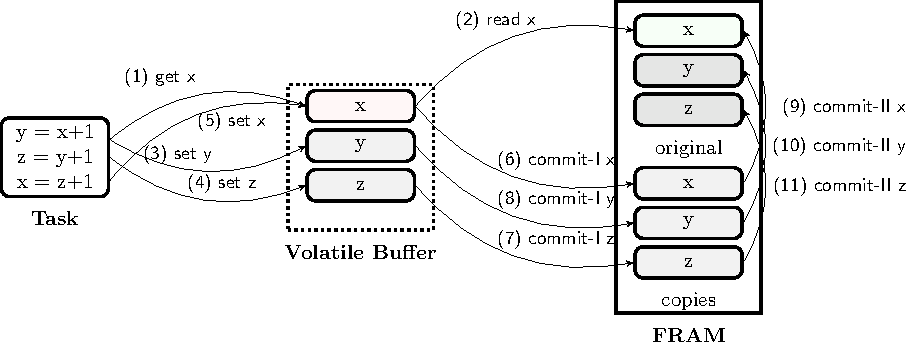
\includegraphics[width=0.75\columnwidth]{figures/sram-buffer}
%	\caption{The interaction between the task, volatile buffer and the non-volatile memory (FRAM). Initially, the persistent variable \texttt{x} is not in the volatile buffer but \texttt{y} and \texttt{z} are.}
%	\label{fig:volatile-buffer}
%\end{figure}

%\subsection{Memory Consistency}

\textbf{Memory Consistency.} \sys's paging mechanism ensures that a task only ever executes using consistent protected data. During task execution, modifications to protected data do not affect their original memory locations, because a task reads and writes the volatile \texttt{working} buffer only, and modified pages are kept in \texttt{\underline{shadow}} until commit.
A power failure erases the contents of the page buffer, preventing a re-executing task from observing updates in the page buffer from a previous execution attempt.
Clearing \texttt{\underline{shadowCount}} as part of the second phase commit (Line 14), ensures that all accesses to protected variables in subsequent tasks correctly access their original memory locations in \texttt{\underline{store}}.
\sys assumes that the write to a non-volatile word in memory is atomic.
%
%The non-volatile commit bit persists
%across power failures and \sys repeatedly attempts to commit until it succeeds,
%despite arbitrary power failures.
\subsection{Dynamic Paging of \sys}

One design choice \sys made was to insert dynamic check for paging on every
possible problematic memory operation using {\tt RP} and {\tt WP} macros.
Since dynamic checks incur overhead on every read and write, it has a higher
overhead for accessing memory than a static approach,
e.g., Alpaca, where a system statically analyze the memory operation and try to insert only optimal
number of memory protection code (usually at the beginning of each task). 

However, \sys's dynamic paging has several benefits over static approach.
First, static approach has limitations, prohibiting certain types of programming pattern. For example,
in the presence of arbitrary pointer operation, function calls using function pointer, or an interrupt
within a task, the system cannot statically analyze the memory behavior. Thus, static
approaches either prohibits the programmer from using certain programming pattern~\cite{alpaca}, 
or will have to conservatively insert memory protection code that can be unnecessary.
Second, static approach cannot handle task coalescing, because with coalescing the scope to be
searched statically is not determined at compile time. 
By choosing to check every memory access dynamically, \sys supports programming pattern that
Alpaca does not support, such as arbitrary pointer operation, while also being able to
support task coalescing, which yields extra performance benefits.
%
%Moreover, if the programmer wants to optimize for high performance, it is possible for the
%programmer to place {\tt RP} and {\tt WP} only minimally by carefully examining the code.
%We argue that the 


%\TODO{Put paragraph about Alpaca's static privatization algo vs. Coala's dynamic privatization algo}
%\TODO{pass by ref might not work the right way}
%\begin{verbatim}
%
%GLOBAL_(x)
%
%foo(*y){ 
%  *y++; 
%}
%
%TASK( ){ 
%  ... ;  
%  foo( &GV(x) ) ; 
%}
%
%\end{verbatim}
%\subsection{Managing Paging Overhead}
%
%The efficiency of \sys's paging scheme relies on the fact that data in pages are contiguous, which makes them amenable to being manipulated by hardware assisted DMA bulk copy operations. To justify this design choice we experimentally evaluated the efficiency of using DMA block copies, compared to explicit, software copy loops. We copied blocks of data of different size between memory regions on a WISP~\cite{wisp} using a hand-written loop and using DMA (refer to Section~\ref{sec:results_hardware} for hardware setup details). Figure~\ref{fig:dmaTimeEnergy} shows that for moving large blocks of data like a page, hardware DMA is considerably better than software in both run time and energy efficiency. \sys's design moves data in pages, not individual words, leveraging the increased efficiency of DMA data movement.
%
%\begin{figure}[t]
%	\centering
%	\subfloat[Time needed to transfer a block of data]{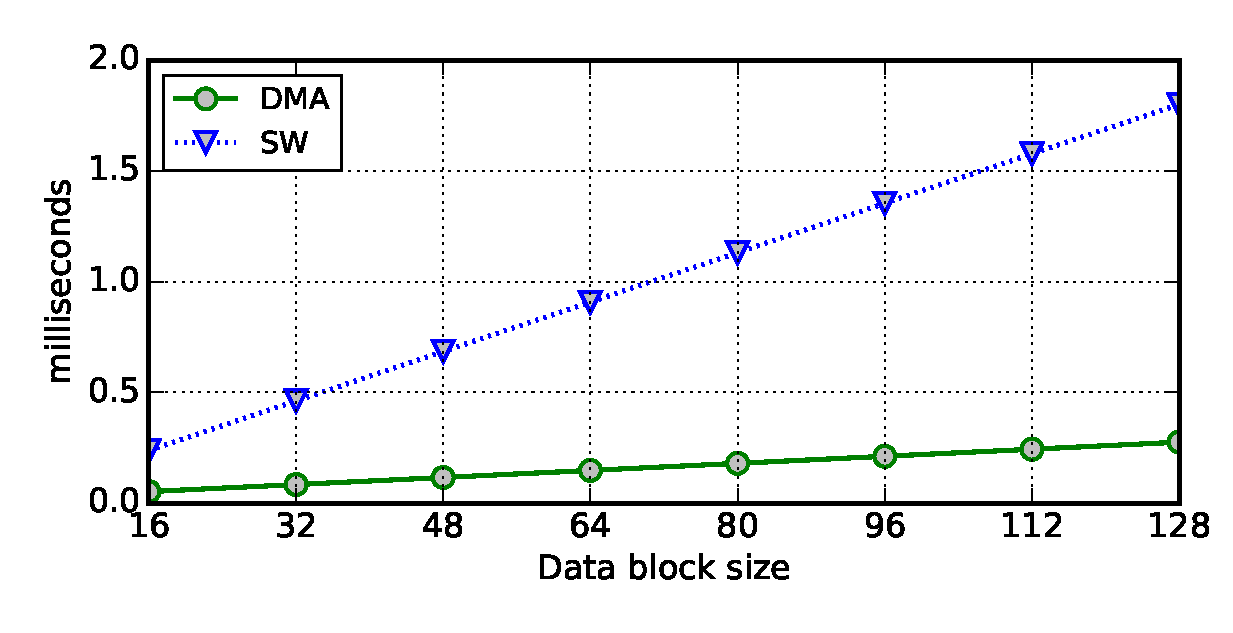
\includegraphics[width=0.49\columnwidth]{figures/dmaSize_time.eps} }
%	\subfloat[Energy needed to transfer a block of data]{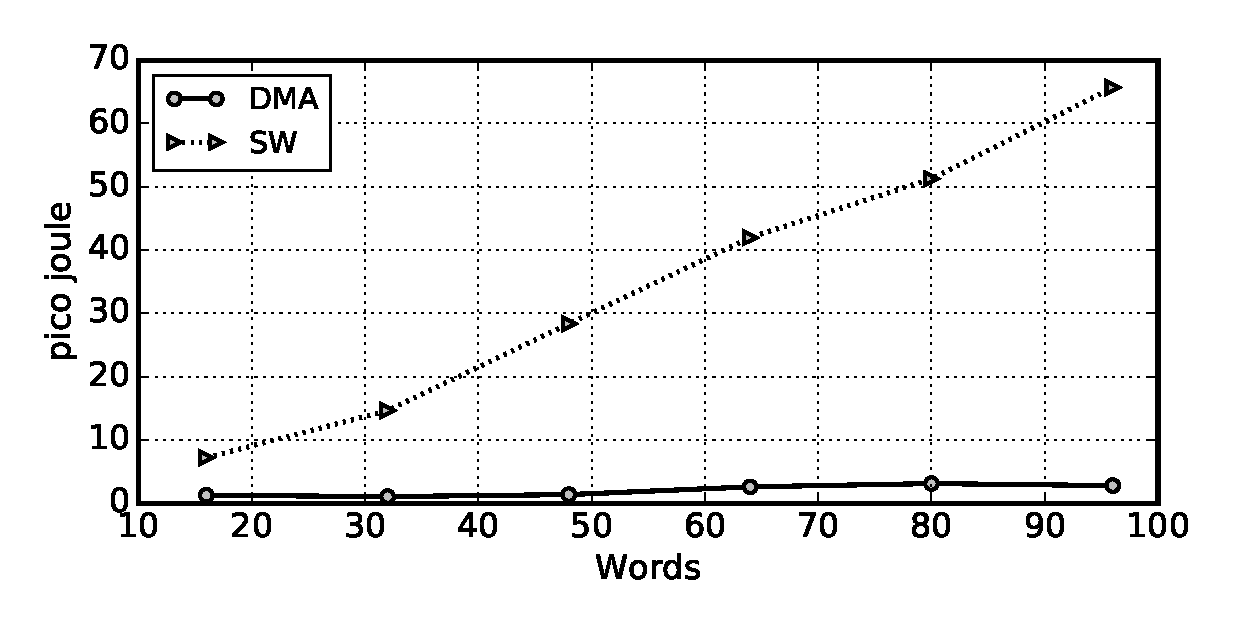
\includegraphics[width=0.49\columnwidth]{figures/energyConsumptionDMA_SW.eps}}
%	\caption{Time and energy consumption of moving a block of data from SRAM to FRAM: CPU intervention versus Direct Memory Access (DMA).\todo{Explain HW/SW setup; make fonts larger, unify legends and axes}{Amjad}}
%	\label{fig:dmaTimeEnergy}
%\end{figure}
